\documentclass[a4paper]{report}
\usepackage[utf8]{inputenc}
\usepackage[ngerman]{babel}
\usepackage{graphicx}
\usepackage[hyphens]{url}
\usepackage[hidelinks]{hyperref}
\usepackage[toc,nonumberlist,style=altlist]{glossaries}
\usepackage{longtable}
\usepackage{caption}
\usepackage{booktabs}
\usepackage{float}
\usepackage{listings}
\usepackage{newclude}


\newenvironment{code}{\ttfamily}{\par}

\begin{document}
\begin{titlepage}
	\centering
	{\scshape\Huge QA-Project}
	\vspace{1cm} \\
	{\scshape\LARGE Web Engineering - PLS}
	\vspace{1cm} \\
	{\scshape\LARGE Handbuch}
	\vspace{1cm} \\
	{\large\itshape Pascal Süß - 72273} \\
	\vspace{0.5cm}
	{\large\itshape Lukas Wallisch - 73242} \\ 
	\vspace{0.5cm}
	{\large\itshape Sebastian Karl - 72138} \\ 
	\vfill
	{\large \today}
\end{titlepage}
\title{Handbuch}

\tableofcontents

\part{Frontend}
\chapter{Design}
Es wurde auf ein möglichst aufgeräumtes Design geachtet, um eine schöne Darstellung, auch auf mobilen Endgeräten, zu ermöglichen. Um den minimalistischen Stil zu verstärken werden Fragen auf der Seite mit Q abgekürzt und Antworten mit A. Zudem wurden auf weitestgehend auf Farbe verzichtet um die Buttons besser hervorzuheben.
\chapter{Bedienung}
\section{Login}
\begin{figure}[h!]
	\centering
	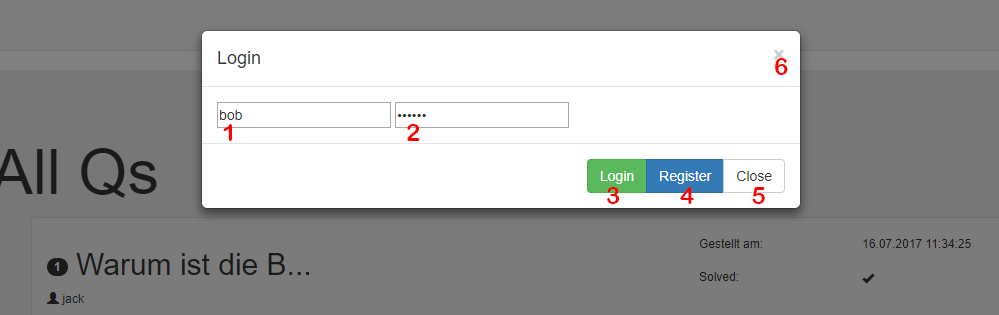
\includegraphics[width=0.9\textwidth]{Login.PNG}
	\caption{Login-/Registrierungsfenster}
	\label{fig:Loginfenster}
\end{figure}
\centering\begin{enumerate}
	\item Login-/Registrierungsname Feld
	\item Passwortfeld
	\item Loginbutton
	\item Registrierbutton
	\item Schließe Anmeldefenster
	\item Schließe Anmeldefenster
\end{enumerate}
\newpage
\section{Grundansicht}
\begin{figure}[h!]
	\centering
	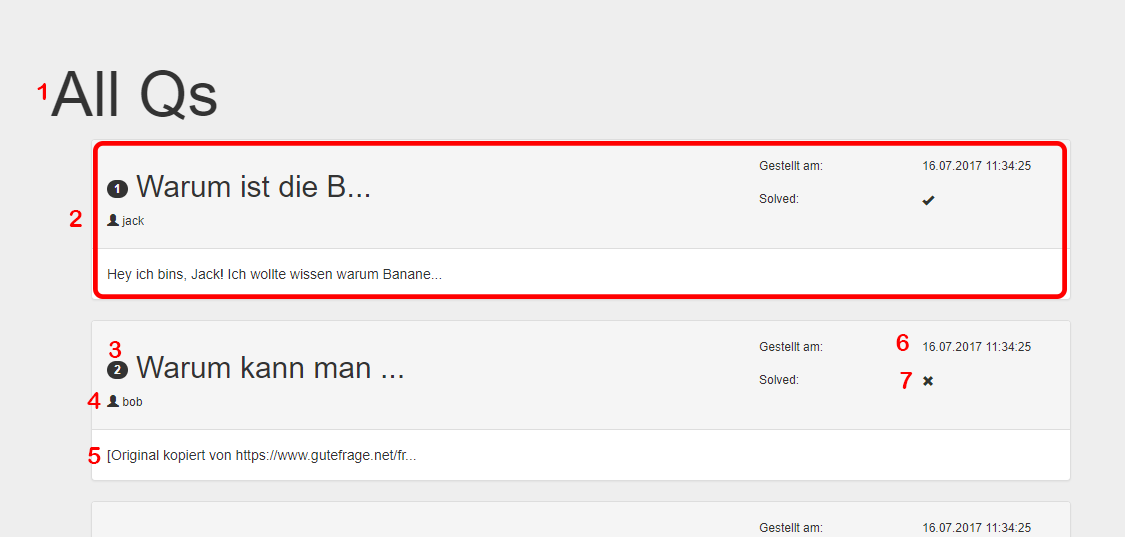
\includegraphics[width=0.9\textwidth]{AlleFragen.PNG}
	\caption{Grundansicht}
	\label{fig:Grundansicht}
\end{figure}
\centering\begin{enumerate}
	\item Welche Fragen werden angezeigt af der aktuellen Ansicht angezeigt
	\item Fragenvorschau, bei klick innerhalb des roten Rechtecks wird die Detailansicht geöffnet.
	\item Anzeige wie viele Antworten es schon zu der Frage gibt
	\item Name des Fragestellers
	\item Vorschau Fragentext max 25 Zeichen
	\item Zeitpunkt der Fragestellung
	\item Anzeige ob eine akzeptierte Antwort zur Frage existiert
\end{enumerate}
\newpage
\section{Detailansicht}
\begin{figure}[h!]
	\centering
	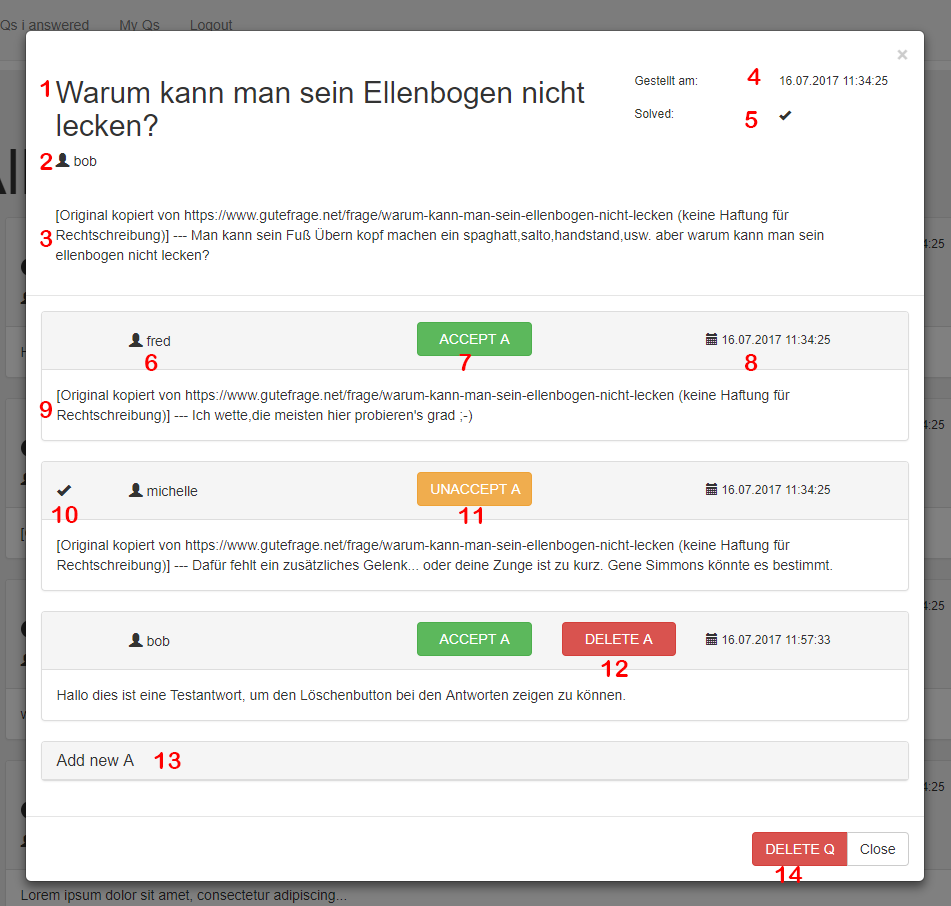
\includegraphics[width=0.9\textwidth]{FrageMitAntworten.PNG}
	\caption{Detailansicht}
	\label{fig:Detailansicht1}
\end{figure}
\centering\begin{enumerate}
	\item Fragentitel
	\item Name des Fragenstellers
	\item Fragentext
	\item Zeitpunkt der Fragestellung
	\item Anzeige ob eine akzeptierte Antwort zur Frage existiert
	\item Name des Antwortgebers
	\item Button zum akzeptieren einer Frage, wird nur dem Fragensteller angezeigt
	\item Zeitpunkt der Antwort
	\item Antworttext
	\item Anzeige ob diese Antwort akzeptiert wurde
	\item Button zum deakzeptieren einer Frage, wird nur dem Fragensteller angezeigt
	\item Button zum löschen einer Frage, wird nur dem jeweiligem Antwortgeber angezeigt
	\item Button der den Antwortdialog öffnet
	\item Button zu Frage löschen, wird nur dem Fragesteller angezeigt. 
\end{enumerate}
\begin{figure}[h!]
	\centering
	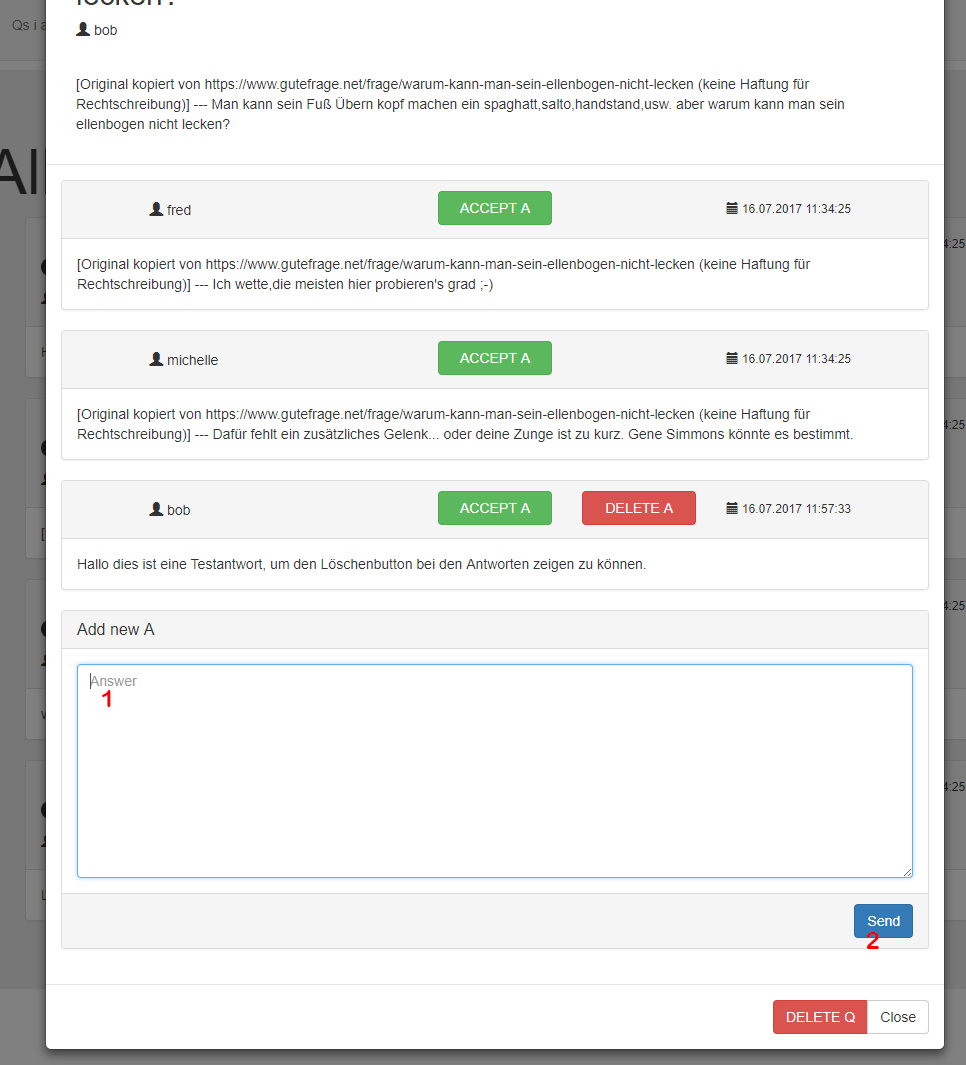
\includegraphics[width=0.9\textwidth]{FrageMitAntwortenUndAntwortfeld.PNG}
	\caption{Detailansicht}
	\label{fig:Detailansicht2}
\end{figure}
\centering\begin{enumerate}	 
	\item Eingabefeld für den Antworttext
	\item Button zum Absenden einer Antwort
\end{enumerate}
\newpage

\section{Neu Frage}
\begin{figure}[h!]
	\centering
	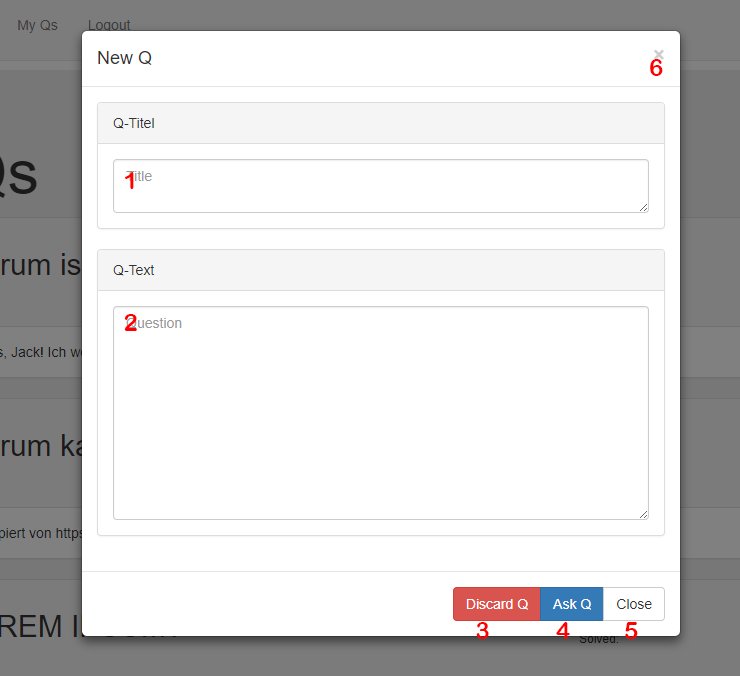
\includegraphics[width=0.9\textwidth]{NewQ.PNG}
	\caption{Neue Frage}
	\label{fig:NeueFrage}
\end{figure}
\centering\begin{enumerate}
	\item Eingabefeld für den Fragentitel
	\item Eingabefeld für den Fragentext
	\item Button zum Löschen aller Eingaben
	\item Button zum versenden der Frage
	\item Button zum Schließen des Fensters
	\item Button zum Schließen des Fensters
\end{enumerate}
\newpage

\section{Navbar}
\begin{figure}[h!]
	\centering
	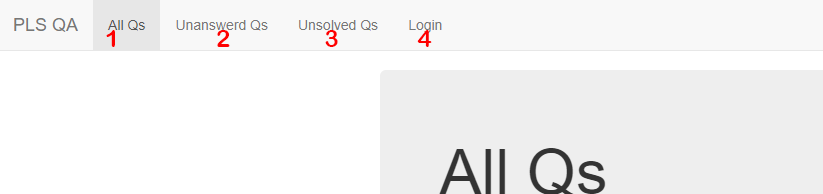
\includegraphics[width=0.9\textwidth]{navbar.PNG}
	\caption{Navbar}
	\label{fig:navbar1}
\end{figure}
\centering\begin{enumerate}
	\item Alle Fragen
	\item Fragen ohne eine Antwort
	\item Fragen ohne eine akzeptierte Antwort
	\item Zeige Logindialog an
\end{enumerate}

\begin{figure}[h!]
	\centering
	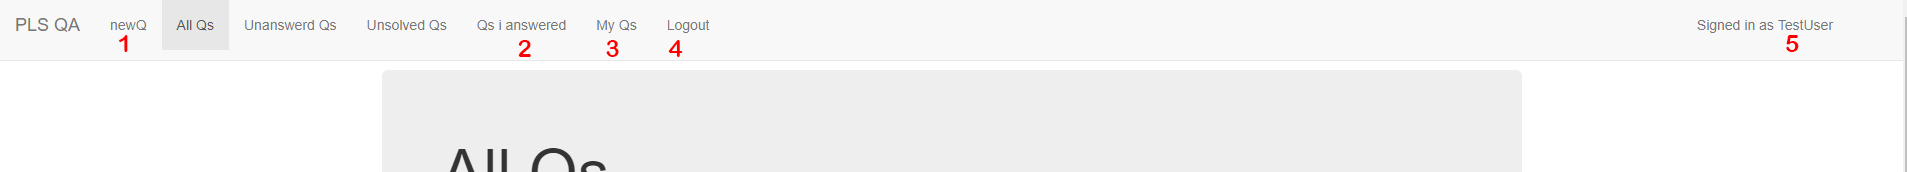
\includegraphics[width=0.9\textwidth]{navbarLoggedIn.PNG}
	\caption{Navbar}
	\label{fig:navbar2}
\end{figure}
\centering\begin{enumerate}
	\item Zeige Neue Fragedialog an
	\item Fragen die ich beantwortet habe
	\item Fragen die von mir gestellt wurden
	\item Logoutbutton
\end{enumerate}

\begin{figure}[h!]
	\centering
	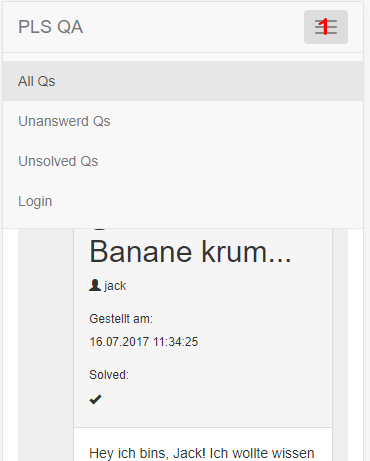
\includegraphics[width=0.3\textwidth]{AnsichtGalaxyS5.PNG}
	\caption{Navbar Galaxy S5 Ansicht}
	\label{fig:navbarResponive}
\end{figure}
\centering\begin{enumerate}
	\item Toggle Menu
\end{enumerate}

\part{Backend}
\chapter{Einfügen von Testdaten}
\label{admin}
Unabhängig von der im Folgenden beschriebenen Einstellung wird ein Admin-Nutzer angelegt, der als einziger Nutzer die Datenbank-Konsole erreichen kann. Die Anmelde-Daten für diesen Nutzer lauten: Username: \textit{admin}, Passwort: \textit{pass}
\section{Ein- und Ausschalten per Konfigurationsdatei}
Der Server generiert standardmäßig Testdaten beim Start. Dies lässt sich verhindern, indem in der \textit{config.properties}, die in der \textit{PLS-Server-1.0.jar} enthalten ist, das \textit{testDataOn}-Flag auf \textit{false} gestellt wird.\\
Alternativ zu \textit{true} und \textit{false} wird folgendes akzeptiert:
\begin{itemize}
	\item \textit{on} und \textit{off}
	\item \textit{yes} und \textit{no}
\end{itemize}
\section{Eingefügte Daten}
Falls die Testdaten generiert werden, werden folgende Nutzer angelegt:
\begin{itemize}
	\item Username: \textit{bob}, Passwort: \textit{bobspw}
	\item Username: \textit{chloe}, Passwort: \textit{cloespw}
	\item Username: \textit{david}, Passwort: \textit{davidspw}
	\item Username: \textit{fred}, Passwort: \textit{fredspw}
	\item Username: \textit{jack}, Passwort: \textit{jackspw}
	\item Username: \textit{kim}, Passwort: \textit{kimspw}
	\item Username: \textit{michelle}, Passwort: \textit{michellespw}
\end{itemize}
Außerdem werden noch 4 Fragen und Antworten angelegt. Dabei ist eine Frage bereits gelöst, eine besitzt noch keine Antworten und die beiden anderen wurden schon beantwortet, allerdings wurde noch keine Antwort akzeptiert.
\chapter{Start der Applikation}
Zum starten der Applikation muss der Befehl \textit{java -jar PLS-Server-1.0.jar} im Verzeichnis in dem sich die .jar-Datei befindet ausgeführt werden. Der Server belegt dabei den Port 8080.
\chapter{Besonderheiten}
\section{Datenbank-Konsole}
\subsection{Aufrufen der Datenbank-Konsole}
Die Datenbank-Konsole ist unter \textit{http://localhost:8080/h2-console} zu erreichen. Um die Konsole aufrufen zu können, sind Admin-Rechte erforderlich(siehe Kapitel~\ref{admin}).\\ 
Wenn vom Browser bereits ein Cookie eines anderen Benutzers gespeichert wurde, wird die Meldung \textit{"You need Admin rights to access this Page!"} angezeigt und es muss ein Login mit dem Admin-Nutzer auf der Client-Seite durchgeführt werden. Wurde kein Cookie gespeichert, wird das Standard HTTP-Basic Anmeldefenster des Browsers erscheinen, in das die Nutzerdaten eingetragen werden müssen.
\subsection{Einloggen in die Datenbank}
Hat man die Datenbank erreicht, muss folgendes in die entsprechenden Felder eingetragen werden:\\

\begin{code}
	Driver Class: org.h2.Driver\\
	JDBC URL: jdbc:h2:mem:testdb\\
	User Name: sa\\
	Password: \\
\end{code}
\noindent
Danach muss nur noch der \textit{Connect}-Kopf gedrückt werden.
\end{document}